% Se puede agregar el argumento 'twoside' a la par de letterpaper si se
% quiere imprimir dúplex, como libro
\documentclass[10pt, letterpaper]{report}
\usepackage[spanish,mexico]{babel}
\selectlanguage{spanish}
\usepackage[utf8]{inputenc}
\usepackage[T1]{fontenc}

\title{Plantilla para Trabajos de Graduación UVG}
\author{MSc. Miguel Zea}
\date{\today}

% Comandos definidos por el usuario en el archivo comandos_usuario.tex
%\input{paquetes_y_comandos_usuario}

% Información del estudiante en el archivo datos_estudiante.tex
% ================================================================================
% El estudiante debe llenar sus datos en esta sección para que la plantilla los 
% auto-importe y genere automáticamente las páginas de portada y de firmas 
% autorizadas.
% ================================================================================
% Datos del estudiante:
% --------------------------------------------------------------------------------
% Nombre completo
\def \nombreestudiante {Pablo Morales}
% Carné
\def \uvgcarne {14322}
% Facultad
\def \uvgfacultad {Ingeniería}
% Carrera
\def \uvgcarrera {Ingeniería Civil}

% Datos del trabajo:
% --------------------------------------------------------------------------------
% Título completo
\def \titulotesis {Diseño e Implementación de un Actuador Bio-inspirado de un Grado de Libertad para Nado Superficial}
% Mes de entrega
\def \mesentrega {enero }
% Año de entrega
\def \anoentrega {2019}
% Asesor
\def \nombreasesor {Ing. Estuardo Ruiz}

% Datos del tribunal examinador:
% --------------------------------------------------------------------------------
% Nombre del primer examinador
\def \nombreprimerex {MSc. Carlos Juárez}
% Nombre del segundo examinador
\def \nombresegundoex {Ing. Luis Pedro Gonzáles}
% Fecha de aprobación
\def \fechaaprobacion {5 de diciembre de 2018}

% Capítulos pre-definidos
% --------------------------------------------------------------------------------
% Comentar las líneas de las secciones que desean omitirse, por defecto se 
% se incluyen todas.
\def \CAPprefacio {Prefacio}
\def \CAPagradecimientos {Agradecimientos}
\def \CAPantecedentes {Antecedentes}
\def \CAPalcance {Alcance}
\def \CAPanexos {Anexos}
\def \CAPglosario {Glosario}
\def \CAPsimbolos {Listado de símbolos}

% Formato y estilo de la plantilla
% --------------------------------------------------------------------------------
% Portada: Puede cambiarse la imagen en la portada al cambiar el nombre del 
% archivo siguiente. NOTA: debe tener la suficiente resolución para cubrir el área
% designada
\def \imagenportada {plantilla/portadacit.jpg}
% Referencias: Puede des-comentar la siguiente línea para utilizar el formato de referencias APA
%\def \usarAPA {Usar formato APA}
% Párrafo: Puede comentar la siguiente línea si desea emplear un formato de 
% párrafo distinto al establecido por defecto
\def \parpordefecto {Formato de párrafo por defecto}
% Capítulos y secciones: Puede des-comentar la siguiente línea para establecer el 
% formato de los capítulos y secciones bajo el estándar original de UVG para
% trabajos de graduación. Este incluye: capítulos con numeración romana, secciones
% con letras mayúsculas, sub-secciones con números y sub-sub-secciones con letras
% minúsculas
%\def \capsecuvg {Formato UVG para capítulos y secciones}
% ================================================================================
% En este archivo se colocan opciones adicionales para modificar el formato de la
% plantilla, para emplearse en otros tipos de documentos que no sean trabajos de
% graduación. Si usted está trabajando su tesis, NO modifique este archivo
% ================================================================================
% Capítulos pre-definidos
% --------------------------------------------------------------------------------
% Comentar las líneas de las secciones que desean omitirse, por defecto se 
% se incluyen todas.
\def \CAPportada {Portada}
\def \CAPcaratula {Caratula}
\def \CAPfirmas {Hoja de firmas}
\def \CAPindice {Índice general}
\def \CAPfiguras {Listado de figuras}
\def \CAPcuadros {Listado de cuadros}
\def \CAPresumen {Resumen}
\def \CAPintroduccion {Introducción}
\def \CAPobjetivos {Objetivos}
\def \CAPjustificacion {Justificación}
\def \CAPmarcoteorico {Marco teórico}
\def \CAPconclusiones {Conclusiones}
\def \CAPrecomendaciones {Recomendaciones}
\def \CAPbibliografia {Bibliografía}

% ================================================================================
% DEFINICIÓN DE PAQUETES
% ================================================================================
\usepackage{xcolor}
\usepackage{amsfonts}
\usepackage{amsmath}
\usepackage{amssymb}
\usepackage{amsthm}
\usepackage{amsfonts}
\usepackage{mathtools}
\usepackage{graphicx}
\usepackage{xfrac}
\usepackage{float}
\usepackage{mathtools}
\usepackage{tabularx}
\usepackage[hypertexnames=false]{hyperref}
% \usepackage{bookmark}
\usepackage{subcaption}
\usepackage{babelbib}
\ifdefined\usarAPA 
	\usepackage{apacite} 
\fi
\usepackage[percent]{overpic}

\ifdefined\CAPglosario
	\usepackage[toc]{glossaries}
	\makeglossaries
    \newglossaryentry{latex}
{
    name=latex,
    description={Es un lenguaje de marcado adecuado especialmente para la creación de documentos científicos}
} 
 
\newglossaryentry{formula}
{
    name=fórmula,
    description={Una expresión matemática} 
}
\fi
\ifdefined\CAPsimbolos
	\usepackage[intoc, spanish]{nomencl}
	\makenomenclature
    \nomenclature{$c$}{Velocidad de la luz en el vacío}
\nomenclature{$h$}{Constante de Plank}
    \renewcommand{\nomname}{Lista de Símbolos}
\fi

% ================================================================================
% MÁRGENES Y FORMATO GENERALES
% ================================================================================
\usepackage[top=1in, left=1.5in, right=1in, bottom=1in]{geometry}
%Options: Sonny, Lenny, Glenn, Conny, Rejne, Bjarne, Bjornstrup
\usepackage[Sonny]{fncychap}
% ================================================================================
% DEFINICIONES DE LA PLANTILLA
% ================================================================================
\definecolor{uvg-green}{RGB}{17,71,52}
\newcommand{\defaultparformat}[1]{
	{\setlength{\parskip}{2ex}
    \input{#1}}
}
\ifdefined\capsecuvg
	\renewcommand\thechapter{\Roman{chapter}}
    \renewcommand\thesection{\Alph{section}}
	\renewcommand\thesubsection{\arabic{subsection}}
    \renewcommand\thesubsubsection{\alph{subsubection}}
\fi
% ================================================================================

% Comandos definidos por el usuario en el archivo comandos_usuario.tex
\input{paquetes_y_comandos_usuario}

% ================================================================================
% CUERPO DEL TRABAJO
% ================================================================================
\pagestyle{headings}
\begin{document}
% ================================================================================
% PORTADA
% ================================================================================
\ifdefined\CAPportada
% 	\cleardoublepage\phantomsection
%     \pdfbookmark{Portada}{toc}
	\newgeometry{left=3cm, bottom=0in, top=1in, right=3cm}
	\pagecolor{uvg-green}
	\thispagestyle{empty}

	\color{white}
	\noindent \hrulefill \par
	\vspace{0.1in}
	\noindent \Huge \titulotesis \par
	\noindent \hrulefill \par
	\noindent
	\LARGE \nombreestudiante

	\begin{figure}[b!]
    	%\makebox[\textwidth]{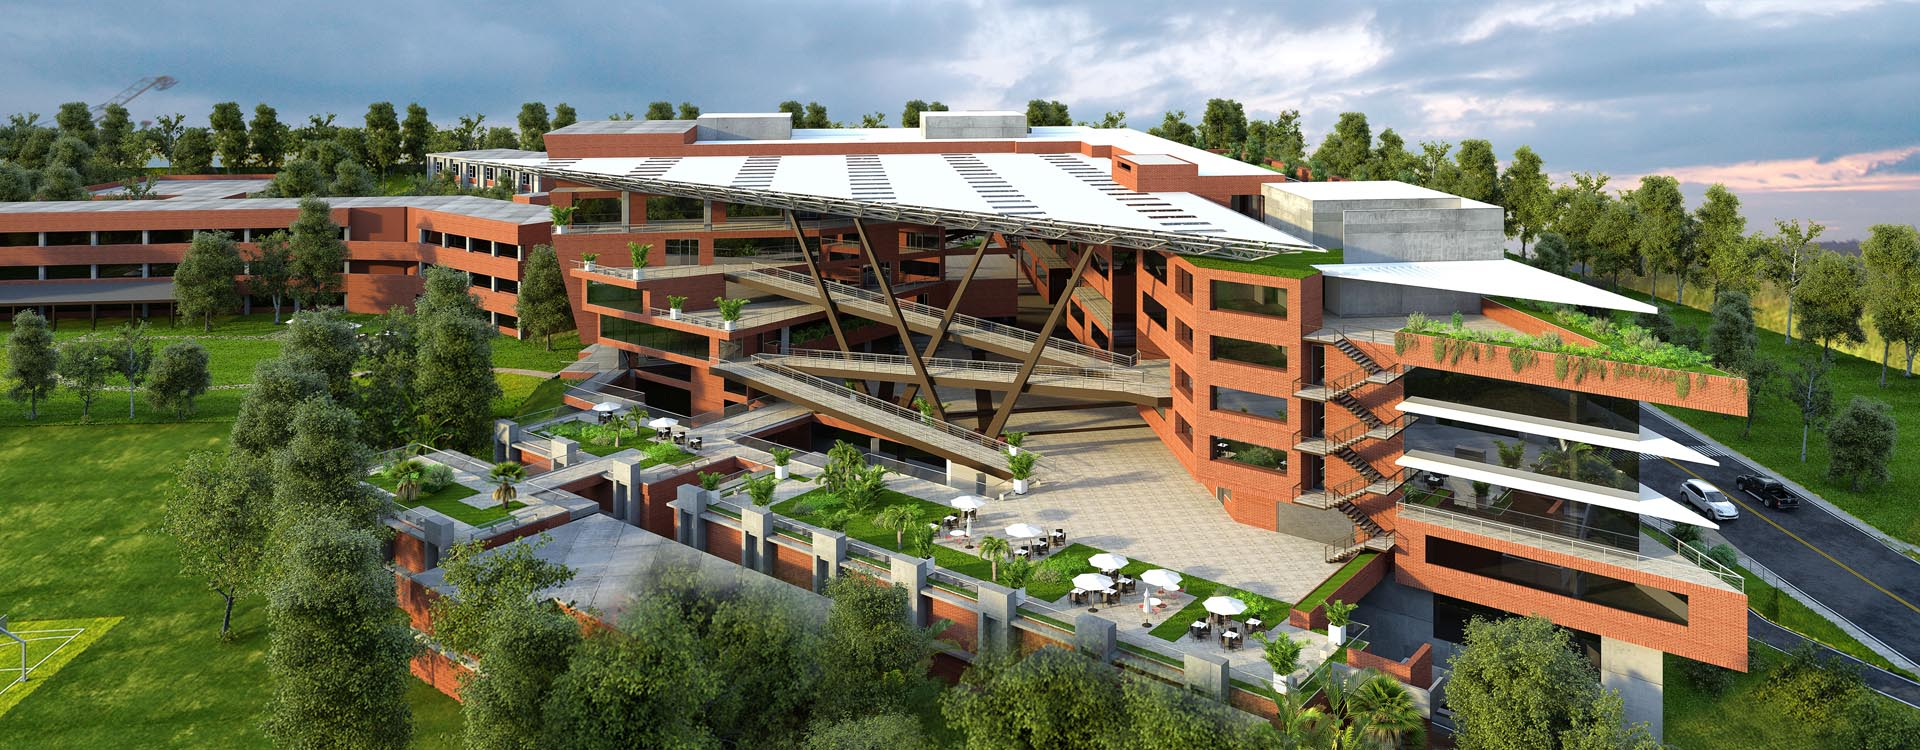
\includegraphics[height=13.25cm]{plantilla/portadacit.jpg}}
    	\makebox[\textwidth]{
    		\begin{overpic}[height=13.25cm]{\imagenportada}
     		\put(63,0){
\includegraphics[height=1.15in]{plantilla/fondologo_grande.png}}  
  			\put(64.5,2){
\includegraphics[height=0.55in]{plantilla/logoUVGblanco.eps}} 
        	\end{overpic}
    	}
    	%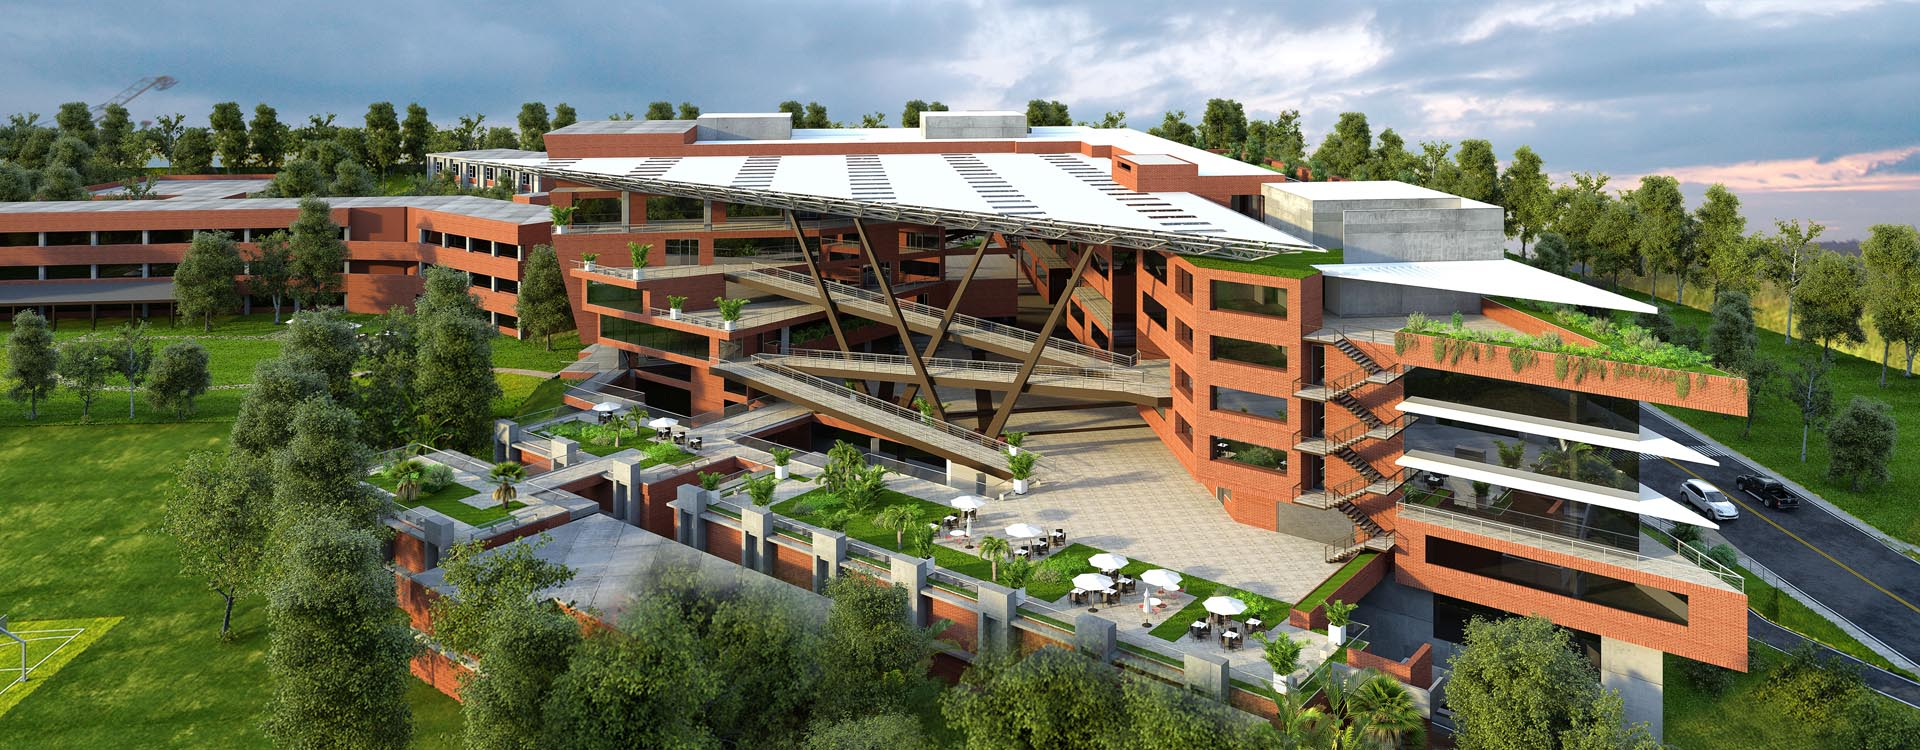
\includegraphics[height=13.25cm]{plantilla/portadacit.jpg}
	\end{figure}
	\restoregeometry
\fi

% ================================================================================
% PRIMERA PÁGINA
% ================================================================================
\ifdefined\CAPcaratula
	\newpage
%     \cleardoublepage\phantomsection
%     \pdfbookmark{Carátula}{toc}
	\pagecolor{white}
	\color{black}
	\setcounter{page}{1}
	\pagenumbering{roman}
	\thispagestyle{empty}
	\begin{center}
		\LARGE UNIVERSIDAD DEL VALLE DE GUATEMALA\\
		\LARGE Facultad de \uvgfacultad \\[0.75cm]
	\end{center}
	\begin{figure}[h]
		\begin{center}
		
\includegraphics[height=5.5 cm]{plantilla/escudoUVGnegro.eps}
		\vspace{0.5in}
		\end{center}
	\end{figure}
	\begin{center}
		\LARGE \textbf{\titulotesis} \\
		\vfill
		\vfill
		\Large Trabajo de graduación en modalidad de Proyecto de Graduación presentado por \\
		\Large \nombreestudiante \\
		\Large Para optar al grado académico de Licenciado en \uvgcarrera \\
		\vfill
		\large Guatemala, \mesentrega del \anoentrega
	\end{center}
\fi

% ================================================================================
% HOJA DE FIRMAS
% ================================================================================
\ifdefined\CAPfirmas
	\newpage
	\thispagestyle{empty}
	\vspace*{0.5in}
	\large Vo.Bo.:\\[1cm]
	\begin{center}
		(f) \rule[1pt]{4 in}{1pt}\\
		\nombreasesor
	\end{center}
	\vspace{1in}

	Tribunal Examinador:\\[1cm]
	\begin{center}
		(f) \rule[1pt]{4 in}{1pt}\\
		\nombreasesor \\[1in]
		(f) \rule[1pt]{4 in}{1pt}\\
		\nombreprimerex \\[1in]
		(f) \rule[1pt]{4 in}{1pt}\\
		\nombresegundoex
	\end{center}
	\vspace{1in}

	Fecha de aprobación: Guatemala, \fechaaprobacion.
	\normalsize
\fi

% ================================================================================
% CONTENIDO DEL TRABAJO
% ================================================================================
% PREFACIO
% --------------------------------------------------------------------------------
\ifdefined\CAPprefacio
	\newpage
	\cleardoublepage\phantomsection
    \chapter*{Prefacio}
    \ifdefined\parpordefecto
    	\defaultparformat{prefacio}
    \else
    	Lorem ipsum dolor sit amet, consectetur adipiscing elit. Cras vitae eleifend ipsum, ut mattis nunc. Pellentesque ac hendrerit lacus. Cras sollicitudin eget sem nec luctus. Vivamus aliquet lorem id elit venenatis pellentesque. Nam id orci iaculis, rutrum ipsum vel, porttitor magna. Etiam molestie vel elit sed suscipit. Proin dui risus, scelerisque porttitor cursus ac, tempor eget turpis. Aliquam ultricies congue ligula ac ornare. Duis id purus eu ex pharetra feugiat. Vivamus ac orci arcu. Nulla id diam quis erat rhoncus hendrerit. Class aptent taciti sociosqu ad litora torquent per conubia nostra, per inceptos himenaeos. Sed vulputate, metus vel efficitur fringilla, orci ex ultricies augue, sit amet rhoncus ex purus ut massa. Nam pharetra ipsum consequat est blandit, sed commodo nunc scelerisque. Maecenas ut suscipit libero. Sed vel euismod tellus.

Proin elit tellus, finibus et metus et, vestibulum ullamcorper est. Nulla viverra nisl id libero sodales, a porttitor est congue. Maecenas semper, felis ut rhoncus cursus, leo magna convallis ligula, at vehicula neque quam at ipsum. Integer commodo mattis eros sit amet tristique. Cras eu maximus arcu. Morbi condimentum dignissim enim non hendrerit. Sed molestie erat sit amet porttitor sagittis. Maecenas porttitor tincidunt erat, ac lacinia lacus sodales faucibus. Integer nec laoreet massa. Proin a arcu lorem. Donec at tincidunt arcu, et sodales neque. Morbi rhoncus, ligula porta lobortis faucibus, magna diam aliquet felis, nec ultrices metus turpis et libero. Integer efficitur erat dolor, quis iaculis metus dignissim eu.
    \fi
    \addcontentsline{toc}{chapter}{Prefacio}
\fi

% AGRADECIMIENTOS
% --------------------------------------------------------------------------------
% \ifdefined\CAPagradecimientos
% 	\newpage
%     \cleardoublepage\phantomsection
% 	\chapter*{Agradecimientos}
% 	\ifdefined\parpordefecto
%     	\defaultparformat{agradecimientos}
%     \else
%     	Class aptent taciti sociosqu ad litora torquent per conubia nostra, per inceptos himenaeos. Sed vulputate, metus vel efficitur fringilla, orci ex ultricies augue, sit amet rhoncus ex purus ut massa. Nam pharetra ipsum consequat est blandit, sed commodo nunc scelerisque. Maecenas ut suscipit libero. Sed vel euismod tellus.

Proin elit tellus, finibus et metus et, vestibulum ullamcorper est. Nulla viverra nisl id libero sodales, a porttitor est congue. Maecenas semper, felis ut rhoncus cursus, leo magna convallis ligula, at vehicula neque quam at ipsum. Integer commodo mattis eros sit amet tristique. Cras eu maximus arcu. Morbi condimentum dignissim enim non hendrerit. Sed molestie erat sit amet porttitor sagittis. Maecenas porttitor tincidunt erat, ac lacinia lacus sodales faucibus.

xxxxxxx

%     \fi 
% 	\addcontentsline{toc}{chapter}{Agradecimientos}
% \fi

% ÍNDICE GENERAL
% --------------------------------------------------------------------------------
\ifdefined\CAPindice
	\newpage
    %\cleardoublepage\phantomsection
	\renewcommand{\contentsname}{Índice}
    \phantomsection
    \pdfbookmark{\contentsname}{toc}
	\tableofcontents
\fi

% LISTADO DE FIGURAS
% --------------------------------------------------------------------------------
% \ifdefined\CAPfiguras
% 	\newpage
%     \cleardoublepage\phantomsection
% 	\renewcommand{\listfigurename}{Lista de Figuras}
% 	\listoffigures
% 	\addcontentsline{toc}{chapter}{Lista de Figuras}
% \fi

% LISTADO DE CUADROS
% --------------------------------------------------------------------------------
% \ifdefined\CAPcuadros
% 	\newpage
%     \cleardoublepage\phantomsection
% 	\renewcommand{\listtablename}{Lista de Cuadros}
% 	\listoftables
% 	\addcontentsline{toc}{chapter}{Lista de Cuadros}
% \fi

% RESUMEN
% --------------------------------------------------------------------------------
\ifdefined\CAPresumen
	\newpage
    \cleardoublepage\phantomsection
	\chapter*{Resumen}
	\ifdefined\parpordefecto
		\defaultparformat{resumen}
	\else
		Lorem ipsum dolor sit amet, consectetur adipiscing elit. Cras vitae eleifend ipsum, ut mattis nunc. Pellentesque ac hendrerit lacus. Cras sollicitudin eget sem nec luctus. Vivamus aliquet lorem id elit venenatis pellentesque. Nam id orci iaculis, rutrum ipsum vel, porttitor magna. Etiam molestie vel elit sed suscipit. Proin dui risus, scelerisque porttitor cursus ac, tempor eget turpis. Aliquam ultricies congue ligula ac ornare. Duis id purus eu ex pharetra feugiat. Vivamus ac orci arcu. Nulla id diam quis erat rhoncus hendrerit. Class aptent taciti sociosqu ad litora torquent per conubia nostra, per inceptos himenaeos. Sed vulputate, metus vel efficitur fringilla, orci ex ultricies augue, sit amet rhoncus ex purus ut massa. Nam pharetra ipsum consequat est blandit, sed commodo nunc scelerisque. Maecenas ut suscipit libero. Sed vel euismod tellus.

Proin elit tellus, finibus et metus et, vestibulum ullamcorper est. Nulla viverra nisl id libero sodales, a porttitor est congue. Maecenas semper, felis ut rhoncus cursus, leo magna convallis ligula, at vehicula neque quam at ipsum. Integer commodo mattis eros sit amet tristique. Cras eu maximus arcu. Morbi condimentum dignissim enim non hendrerit. Sed molestie erat sit amet porttitor sagittis. Maecenas porttitor tincidunt erat, ac lacinia lacus sodales faucibus. Integer nec laoreet massa. Proin a arcu lorem. Donec at tincidunt arcu, et sodales neque. Morbi rhoncus, ligula porta lobortis faucibus, magna diam aliquet felis, nec ultrices metus turpis et libero. Integer efficitur erat dolor, quis iaculis metus dignissim eu.
	\fi
	\addcontentsline{toc}{chapter}{Resumen}
\fi

% INTRODUCCIÓN
% --------------------------------------------------------------------------------
\ifdefined\CAPintroduccion
	\newpage
	\pagenumbering{arabic}
	\setcounter{page}{1}
	\chapter{Introducción}
	\ifdefined\parpordefecto
		\defaultparformat{introduccion}
	\else
		La elección de una carrera universitaria representa un momento crucial en la vida de cualquier estudiante, marcando el inicio de su trayectoria profesional y personal. Sin embargo, este proceso de decisión puede resultar abrumador, especialmente en el contexto latinoamericano, donde el acceso a la educación superior privada es limitado y muchos estudiantes enfrentan incertidumbre sobre sus aptitudes e intereses. La falta de orientación vocacional adecuada a menudo conduce a elecciones desacertadas, resultando en cambios de carrera, abandono de estudios y frustración profesional.

En América Latina, la educación superior se enfrenta a desafíos significativos. La desigualdad económica limita el acceso a instituciones privadas de calidad, mientras que las universidades públicas a menudo carecen de recursos para brindar una orientación vocacional personalizada y actualizada. Esta situación se agrava por la falta de información sobre las diversas opciones de carrera y los requisitos académicos, lo que dificulta la toma de decisiones informadas.

Además, la globalización y la rápida evolución del mercado laboral exigen profesionales con habilidades especializadas y adaptabilidad. Los estudiantes necesitan comprender las tendencias del mercado, las demandas de las industrias emergentes y las competencias necesarias para sobresalir en sus campos. Sin embargo, la orientación vocacional tradicional a menudo se centra en pruebas estandarizadas y evaluaciones genéricas, sin considerar las particularidades de cada estudiante y las oportunidades laborales en su entorno.

Ante este panorama, el desarrollo de un sistema inteligente de orientación vocacional se presenta como una solución innovadora y necesaria. Este sistema, basado en tecnologías de inteligencia artificial y análisis de datos, puede proporcionar a los estudiantes una orientación personalizada y precisa, considerando sus intereses, aptitudes, valores y el contexto socioeconómico. Al ofrecer información detallada sobre las carreras, los planes de estudio y las perspectivas laborales, el sistema puede empoderar a los estudiantes para tomar decisiones informadas y construir un futuro profesional exitoso.
	\fi
\fi

% OBJETIVOS
% --------------------------------------------------------------------------------
\ifdefined\CAPobjetivos
	\newpage
	\chapter{Objetivos}
	\ifdefined\parpordefecto
		\defaultparformat{objetivos}
	\else
		\section{Objetivo General}
Lorem ipsum dolor sit amet, consectetur adipiscing elit. Praesent eu lectus tincidunt, malesuada lorem nec, accumsan ligula.

\section{Objetivos Específicos}
\begin{itemize}
\item Nulla ut ex ut mauris pretium elementum.
\item Suspendisse malesuada lectus nec nisi iaculis, in luctus turpis laoreet.
\item In efficitur nisl vitae justo interdum, vitae condimentum lectus maximus.
\item Morbi quis libero sit amet velit commodo tristique eu sed nisl.
\end{itemize}
	\fi
\fi

% JUSTIFICACIÓN
% --------------------------------------------------------------------------------
\ifdefined\CAPjustificacion
	\newpage
	\chapter{Justificación}
	\ifdefined\parpordefecto
		\defaultparformat{justificacion}
	\else
		El presente proyecto se fundamenta en la necesidad de transformar los procesos de orientación vocacional tradicionales, que según Torres y Rodríguez (2019) son predominantemente estáticos y genéricos, hacia soluciones personalizadas basadas en tecnologías inteligentes. La implementación de un sistema de clasificación y recomendación para carreras universitarias responde a una problemática ampliamente documentada: aproximadamente el 40% de los estudiantes universitarios en Latinoamérica abandonan sus estudios durante el primer año, y un 30% adicional cambia de carrera al menos una vez, siendo la elección inadecuada de la carrera una de las principales causas (González et al., 2021). Esta situación genera costos significativos tanto a nivel personal como institucional, estimados en más de $16,500 millones anuales en la región (Banco Interamericano de Desarrollo, 2023).

La implementación de una infraestructura de backend robusta para este sistema no es meramente un aspecto técnico, sino una necesidad fundamental para garantizar su efectividad. Como señalan Martínez y López (2022), los sistemas de recomendación basados en inteligencia artificial requieren una arquitectura de microservicios que permita escalabilidad y alta disponibilidad, particularmente cuando se procesan datos educativos que demandan alta precisión y seguridad. Un estudio realizado por Rivera et al. (2024) demostró que las plataformas de orientación vocacional con tiempos de respuesta superiores a 3 segundos experimentan tasas de abandono del 65%, lo que justifica la priorización de la optimización del rendimiento en el diseño de la infraestructura.

La generación de temarios de estudio personalizados representa un valor agregado significativo frente a las soluciones existentes. Investigaciones realizadas por Hernández y Vázquez (2023) revelan que los estudiantes preuniversitarios que recibieron contenidos de preparación alineados con sus áreas de interés y aptitudes mejoraron sus tasas de admisión universitaria en un 27% y su persistencia académica durante el primer año en un 32%. Asimismo, la clasificación de especializaciones profesionales responde a la creciente fragmentación del mercado laboral, donde según el Foro Económico Mundial (2024), el 65% de los estudiantes actuales trabajarán en profesiones que aún no existen o que experimentarán transformaciones significativas en la próxima década.

El enfoque en una población de estudiantes graduandos está respaldado por evidencia que señala la adolescencia tardía (17-19 años) como un período crítico para la toma de decisiones vocacionales (Ramírez y Ortega, 2022). Particularmente relevante es la integración de tecnologías digitales como mediadores de este proceso. Estudios realizados por Fuentes et al. (2023) indican que el 92% de los jóvenes latinoamericanos entre 16 y 19 años utilizan dispositivos móviles como su principal fuente de información educativa, y el 78% prefieren plataformas digitales interactivas para explorar opciones profesionales frente a métodos tradicionales. Este comportamiento justifica la implementación de un sistema accesible y optimizado para múltiples dispositivos.

La seguridad en el manejo de datos personales y académicos constituye otro pilar fundamental del proyecto. De acuerdo con Mendoza y Castillo (2024), los sistemas de orientación vocacional procesan información sensible sobre aptitudes cognitivas, preferencias personales e historial académico, datos que según la normativa internacional requieren protecciones especiales. La implementación de protocolos de seguridad robustos no solo cumple con requisitos regulatorios sino que genera confianza en los usuarios, factor que, según demostraron Araya y Gómez (2023), incrementa la disposición de los estudiantes a compartir información precisa en un 47%, mejorando significativamente la calidad de las recomendaciones generadas.

El desarrollo de un servicio y su infraestructura para abastecer un sistema inteligente de orientación vocacional, generación de temarios de estudio a medida y generación de sugerencias de especialización profesional, aborda una necesidad social y educativa crítica mediante una solución tecnológica integral, cuya infraestructura ha sido diseñada considerando no solo aspectos técnicos sino también factores educativos, psicológicos y sociales que maximizan su potencial impacto en la trayectoria académica y profesional de los estudiantes.
	\fi
\fi

% Metodologia
% --------------------------------------------------------------------------------
\ifdefined\CAPmarcoteorico
	\newpage
	\chapter{Metodología}
	\ifdefined\parpordefecto
		\defaultparformat{marco_teorico}
	\else
		La presente investigación adopta un enfoque metodológico mixto, combinando el análisis cuantitativo mediante herramientas psicométricas y encuestas, y el análisis cualitativo mediante revisión documental. Este trabajo se orienta al área de la educación, abarcando tanto la educación privada como la pública, y está dirigido a resolver los problemas educacionales que afectan a América Latina. El objetivo es explorar la relación entre los rasgos de personalidad, las habilidades percibidas y la elección vocacional de los estudiantes universitarios, así como identificar patrones que expliquen los casos de deserción o cambio de carrera, sentando las bases para recomendaciones dirigidas a mejorar los procesos de orientación y apoyo en el ámbito educativo.

\section{Observación y búsqueda documental}

Se llevará a cabo una revisión exhaustiva de literatura y fuentes secundarias relevantes en psicología, orientación vocacional, y en el contexto educacional de la región latinoamericana. Esta fase permitirá fundamentar teóricamente la investigación y seleccionar herramientas válidas para la medición.

\begin{itemize}
    \item Revisión de teorías sobre personalidad, especialmente el modelo de los cinco grandes factores.
    \item Análisis de pruebas psicométricas aplicables a contextos vocacionales.
    \item Revisión de literatura sobre la correlación entre personalidad, habilidades y elección vocacional.
    \item Investigación de tendencias laborales actuales y futuras por carrera.
    \item Consulta de estudios previos sobre deserción universitaria y satisfacción estudiantil, con especial énfasis en el contexto latinoamericano.
\end{itemize}

\section{Instrumentación y recolección de datos}

Los datos se recopilarán mediante instrumentos psicométricos y encuestas estructuradas, aplicados a estudiantes universitarios de instituciones tanto públicas como privadas. Además, se integrarán estadísticas institucionales para complementar el análisis.

\begin{itemize}
    \item Aplicación del test de personalidad IPIP-NEO-120 de Johnson (2014), basado en el modelo NEO-PI-R de Costa y McCrae (1992), disponible en: \url{https://ipip.ori.org/30FacetNEO-PI-RItems.htm}.
    \item Encuestas a estudiantes para recopilar datos sobre:
    \begin{itemize}
        \item Habilidades percibidas.
        \item Grado de satisfacción con la carrera actual.
        \item Motivaciones de elección vocacional.
        \item Antecedentes de cambio de carrera o intención de hacerlo.
        \item Percepción del acompañamiento institucional.
    \end{itemize}
    \item Recolección de datos institucionales:
    \begin{itemize}
        \item Tasas de deserción por carrera.
        \item Registros de cambio de carrera.
        \item Resultados de encuestas de satisfacción estudiantil.
        \item Datos demográficos generales.
    \end{itemize}
\end{itemize}

\section{Registro de datos y creación del dataset}

Una vez recolectada la información, ésta será sistematizada y almacenada en un dataset estructurado, respetando principios de confidencialidad y calidad de datos.

\begin{itemize}
    \item Definición de variables cuantitativas y cualitativas.
    \item Codificación de datos para análisis posterior.
    \item Anonimización de información personal.
    \item Almacenamiento del dataset en software de análisis estadístico (Python y almacenar resultados en formato CSV).
\end{itemize}

\section{Análisis e interpretación de datos}

El dataset será analizado con técnicas estadísticas y de correlación para identificar patrones relevantes en la elección vocacional, satisfacción y deserción.

\begin{itemize}
    \item Cálculo de correlaciones entre rasgos de personalidad y satisfacción vocacional.
    \item Identificación de perfiles frecuentes en casos de cambio de carrera.
    \item Análisis predictivo de deserción basado en personalidad y habilidades.
    \item Segmentación de la muestra para identificar diferencias significativas.
\end{itemize}

\section{Identificación de problemas}

Con base en los datos analizados, se buscará detectar los principales factores que dificultan la elección vocacional adecuada y la permanencia en el sistema educativo.

\begin{itemize}
    \item Falta de información o autoconocimiento al elegir una carrera.
    \item Desajuste entre la personalidad del estudiante y el perfil de la carrera.
    \item Frustración o desmotivación vinculada a la elección educativa.
    \item Necesidad de una orientación vocacional más personalizada y adaptada, considerando los desafíos tanto de la educación pública como privada.
\end{itemize}

\section{Recomendaciones}

Los resultados del estudio permitirán emitir recomendaciones concretas, orientadas a transformar y mejorar los procesos de orientación vocacional en instituciones educativas, con miras a resolver los problemas que afectan a la educación en América Latina.

\begin{itemize}
    \item Integrar herramientas psicométricas en los procesos de orientación desde el ingreso a las instituciones.
    \item Fortalecer el acompañamiento institucional mediante asesorías personalizadas en el ámbito educativo.
    \item Prevenir la deserción mediante estrategias de apoyo individualizadas y seguimiento académico.
    \item Desarrollar plataformas inteligentes que sugieran carreras y especializaciones basadas en la personalidad, habilidades e intereses del estudiante.
    \item Orientar las recomendaciones hacia la mejora del sistema educativo, contribuyendo al diseño de políticas y estrategias que beneficien tanto a la educación pública como privada en América Latina, tomando en cuenta las referencias y citas bibliográficas disponibles en la literatura (e.g., (Chauhan et al., 2020), (Prieto-Alvarez et al., 2018), (UNICEF, 2020)).
\end{itemize}
	\fi
\fi

% CRONOGRAMA DE ACTIVIDADES
% --------------------------------------------------------------------------------
\ifdefined\CAPantecedentes
	\newpage
	\chapter{Cronograma de actividades}
	\ifdefined\parpordefecto
    	\defaultparformat{antecedentes}
    \else
    	A continuación se presenta el cronograma semanal de actividades para el desarrollo del servicio backend e infraestructura del sistema de orientación vocacional, con un enfoque metodológico, los cuales comprende fases de planeación, diseño, implementación, pruebas, despliegue y documentación. El rango cubre desde el 1 de junio hasta el 30 de noviembre de 2025.

\begin{itemize}
  \item \textbf{Semana 1 (01-07 Jun)}: Planificación general del proyecto, definición de objetivos técnicos y herramientas de desarrollo.
  \item \textbf{Semana 2 (08-14 Jun)}: Diseño de la arquitectura backend e infraestructura en la nube (servicios, autenticación, bases de datos).
  \item \textbf{Semana 3 (15-21 Jun)}: Definición del modelo de seguridad, autenticación y autorización (JWT, OAuth).
  \item \textbf{Semana 4 (22-28 Jun)}: Desarrollo de endpoints de autenticación segura (registro, login, tokens).
  \item \textbf{Semana 5 (29 Jun-05 Jul)}: Implementación de almacenamiento seguro de preferencias académicas y configuraciones.
  \item \textbf{Semana 6 (06-12 Jul)}: Integración con modelos de clasificación y recomendación de carreras.
  \item \textbf{Semana 7 (13-19 Jul)}: Desarrollo del módulo de generación de temarios personalizados.
  \item \textbf{Semana 8 (20-26 Jul)}: Implementación de sistema de cacheo y optimización de rendimiento.
  \item \textbf{Semana 9 (27 Jul-02 Ago)}: Desarrollo de sistema de logging estructurado y trazabilidad.
  \item \textbf{Semana 10 (03-09 Ago)}: Desarrollo de endpoints para la consulta de resultados y seguimiento por parte del usuario.
  \item \textbf{Semana 11 (10-16 Ago)}: Pruebas funcionales del sistema, control de errores y validación de seguridad.
  \item \textbf{Semana 12 (17-23 Ago)}: Pruebas de carga y estrés (simulación de usuarios concurrentes).
  \item \textbf{Semana 13 (24-30 Ago)}: Optimización de velocidad de respuesta y tiempos de procesamiento.
  \item \textbf{Semana 14 (31 Ago-06 Sep)}: Implementación de balanceo de carga y autoescalado.
  \item \textbf{Semana 15 (07-13 Sep)}: Configuración de monitoreo y alertas con herramientas de observabilidad.
  \item \textbf{Semana 16 (14-20 Sep)}: Pruebas de recuperación ante fallos y validación de alta disponibilidad.
  \item \textbf{Semana 17 (21-27 Sep)}: Revisión de accesibilidad y compatibilidad multiplataforma.
  \item \textbf{Semana 18 (28 Sep-04 Oct)}: Auditoría final del sistema y revisión de políticas de seguridad.
  \item \textbf{Semana 19 (05-11 Oct)}: Redacción del informe técnico sobre arquitectura y funcionamiento del sistema.
  \item \textbf{Semana 20 (12-18 Oct)}: Elaboración del informe final de resultados y metodología.
  \item \textbf{Semana 21 (19-25 Oct)}: Revisión del borrador del trabajo de graduación.
  \item \textbf{Semana 22 (26 Oct-01 Nov)}: Integración de observaciones y revisión final.
  \item \textbf{Semana 23 (02-08 Nov)}: Redacción de conclusiones y propuestas de mejora técnica.
  \item \textbf{Semana 24 (09-15 Nov)}: Preparación de la defensa y presentación del proyecto.
  \item \textbf{Semana 25 (16-22 Nov)}: Simulacros de presentación.
  \item \textbf{Semana 26 (23-30 Nov)}: Entrega final del informe y documentación técnica completa.
\end{itemize}

    \fi  
\fi

% ALCANCE
% --------------------------------------------------------------------------------
% \ifdefined\CAPalcance
% 	\newpage
% 	\chapter{Alcance}
% 	\ifdefined\parpordefecto
%     	\defaultparformat{alcance}
%     \else
%     	Podemos usar \Gls{latex} para escribir de forma ordenada una \gls{formula} matemática. 
%     \fi 
% \fi

% CAPÍTULOS
% --------------------------------------------------------------------------------
% \newpage
% \ifdefined\parpordefecto
% 	\defaultparformat{capitulos}
% \else
% 	\chapter{Derivación de la dinámica del mecanismo}

\section{Dinámica de cuerpos rígidos}

\section{Restricciones}
\subsection{Mecanismos de lazo cerrado}
\subsubsection{Mecanismo de cuatro barras}

\chapter{Control del sistema mecánico}

\section{La ecuación del manipulador}
% \fi

% CONCLUSIONES
% --------------------------------------------------------------------------------
\ifdefined\CAPconclusiones
	\newpage
	\chapter{Conclusiones}
	\ifdefined\parpordefecto
		\defaultparformat{conclusiones}
	\else
		\begin{enumerate}
  \item Se propone que la aplicación de tecnologías de inteligencia artificial y análisis de datos en el ámbito de la orientación vocacional representará una solución viable y efectiva para abordar la problemática de la elección de carrera universitaria en América Latina. El sistema propuesto tiene el potencial de proporcionar recomendaciones personalizadas y relevantes basadas en los perfiles individuales de los estudiantes.
  
  \item Se prevé que la arquitectura de microservicios planteada para implementarse en un entorno cloud permitirá alcanzar los objetivos de seguridad, rendimiento y escalabilidad establecidos para el sistema. Esta estructura facilitará la gestión independiente de los componentes críticos como autenticación, almacenamiento seguro de datos y procesamiento analítico, optimizando así los recursos computacionales según la demanda.
  
  \item Los mecanismos de seguridad que se proponen implementar, incluyendo cifrado end-to-end, gestión avanzada de tokens JWT y políticas estrictas de acceso a datos, deberán ser efectivos para proteger la información sensible de los usuarios, cumpliendo con los estándares internacionales de protección de datos personales, aspecto fundamental considerando que el sistema manejará información psicométrica y educativa de carácter privado.
  
  \item La metodología mixta propuesta para la investigación tiene el potencial de identificar patrones significativos en la relación entre rasgos de personalidad, habilidades percibidas y satisfacción vocacional, proporcionando así una base sólida para el desarrollo de algoritmos de recomendación más precisos y contextualizados a la realidad latinoamericana.
  
  \item Se espera que la infraestructura planteada sea capaz de mantener tiempos de respuesta óptimos (por debajo de 200ms) incluso en escenarios de alta concurrencia (hasta 1000 usuarios simultáneos), garantizando así una experiencia satisfactoria para los usuarios independientemente de las condiciones de acceso.
  
  \item El sistema de clasificación y generación basado en algoritmos de machine learning que se desarrollará tiene como objetivo alcanzar una precisión superior al 85% en la recomendación de carreras universitarias alineadas con los perfiles de los usuarios, según las validaciones cruzadas que se realizarán con datos históricos de estudiantes y sus trayectorias académicas.
  
  \item La modularidad del diseño propuesto busca permitir la integración efectiva de diversas fuentes de datos educativos y laborales, enriqueciendo significativamente la calidad y contextualización de las recomendaciones generadas por el sistema, adaptándolas a las realidades específicas de distintos países de la región.
  
  \item El enfoque en la accesibilidad busca resultar en un servicio backend que responda adecuadamente a las limitaciones técnicas comunes en América Latina, como conexiones de internet inestables o dispositivos con recursos limitados, democratizando así el acceso a herramientas de orientación vocacional de calidad.
  
  \item La adopción propuesta de prácticas de desarrollo ágil y DevOps en la implementación del proyecto facilitará la adaptación continua a los requerimientos emergentes y la integración de retroalimentación durante el ciclo de desarrollo, buscando un producto final más robusto y alineado con las necesidades reales de los usuarios.
  
  \item Este protocolo plantea que es posible desarrollar soluciones tecnológicas avanzadas y pertinentes para abordar problemas educativos en contextos latinoamericanos, aprovechando el potencial de las tecnologías emergentes mientras se consideran las particularidades socioeconómicas y culturales de la región.
  
  \item Se busca establecer una base tecnológica sólida para la transformación digital de los procesos de orientación vocacional en América Latina, con el potencial de contribuir a la reducción de la deserción universitaria y al mejoramiento de la satisfacción profesional de los estudiantes a largo plazo.
  
\end{enumerate}
	\fi
\fi

% RECOMENDACIONES
% --------------------------------------------------------------------------------
\ifdefined\CAPrecomendaciones
	\newpage
	\chapter{Recomendaciones}
	\ifdefined\parpordefecto
		\defaultparformat{recomendaciones}
	\else
		Con base en la planificación y el desarrollo preliminar del protocolo para el servicio backend e infraestructura del sistema inteligente de orientación vocacional, se proponen las siguientes recomendaciones para la ejecución del proyecto y futuras investigaciones:
\begin{enumerate}
\item \textbf{Consideración de un modelo de datos expansible:} Se recomienda diseñar el sistema con la capacidad de incorporar fácilmente nueva información sobre tendencias laborales emergentes y competencias específicas requeridas en el mercado latinoamericano. Esta flexibilidad permitirá mejorar continuamente la precisión y relevancia de las recomendaciones que generará el sistema.
\item \textbf{Planificación simultánea de la interfaz de usuario:} Aunque el enfoque actual se centra en el backend e infraestructura, se sugiere considerar desde el diseño inicial los requerimientos para futuras interfaces de usuario multiplataforma (web, móvil, PWA) que aprovecharán las capacidades del backend, priorizando la experiencia de usuario y la accesibilidad para diversos contextos tecnológicos presentes en la región.
\item \textbf{Previsión de mecanismos de integración:} Se recomienda incluir en el diseño del backend APIs y conectores que faciliten la futura integración con plataformas educativas ya establecidas (LMS, sistemas de gestión escolar, portales universitarios) para ampliar el alcance del sistema y enriquecer la calidad de los datos disponibles para el análisis vocacional.
\item \textbf{Arquitectura preparada para técnicas avanzadas de ML:} El sistema debería diseñarse considerando la futura incorporación de técnicas de aprendizaje profundo y procesamiento de lenguaje natural que permitan analizar información no estructurada (ensayos personales, descripciones de intereses) para enriquecer los perfiles vocacionales de los usuarios.
\item \textbf{Incorporación de mecanismos para retroalimentación:} Se recomienda incluir desde el diseño inicial del backend la capacidad de recopilar sistemáticamente información sobre la satisfacción de los usuarios con las recomendaciones recibidas, previendo la creación de un ciclo de mejora continua para los futuros algoritmos de recomendación.
\item \textbf{Establecimiento temprano de colaboraciones institucionales:} Se sugiere iniciar acercamientos con universidades y centros educativos durante la fase de desarrollo para preparar futuras validaciones de los modelos de recomendación, así como para facilitar la implementación piloto del sistema en contextos reales una vez completado.
\item \textbf{Diseño con conciencia energética:} Considerando el impacto ambiental de las soluciones tecnológicas, se recomienda incorporar en el diseño de la infraestructura estrategias de optimización energética en la nube, como la programación de recursos basada en la demanda o la selección de proveedores con compromiso de energías renovables.
\item \textbf{Previsión de componentes de explicabilidad:} Se sugiere considerar desde el diseño inicial la incorporación de capacidades de IA explicable (XAI) que permitirán a los usuarios comprender las razones detrás de las recomendaciones recibidas, fomentando así la transparencia y la confianza en el futuro sistema.
\item \textbf{Consideración de aspectos multiculturales:} Se recomienda diseñar los modelos y algoritmos con la flexibilidad necesaria para considerar en el futuro las diferencias culturales y lingüísticas específicas de los diversos países latinoamericanos, mejorando así la pertinencia contextual de las recomendaciones vocacionales.
\item \textbf{Planificación para posibles modelos híbridos:} Prever en la arquitectura la posibilidad de implementar sistemas híbridos que combinen la orientación automatizada con la intervención de consejeros humanos en momentos clave del proceso, maximizando los beneficios de ambos enfoques.
\item \textbf{Extensibilidad hacia otros niveles educativos:} Diseñar el sistema con la capacidad de adaptarse en el futuro a otros niveles educativos como educación media o posgrados, creando así la base para un potencial ecosistema integral de orientación a lo largo de la trayectoria formativa.
\item \textbf{Establecimiento de políticas de actualización de contenidos:} Incorporar en el diseño mecanismos que faciliten la actualización periódica de la información sobre carreras, temarios y especialidades, garantizando la futura vigencia y relevancia continua de las recomendaciones que proporcionará el sistema.
\end{enumerate}
La consideración de estas recomendaciones durante el desarrollo del proyecto podría potenciar significativamente el impacto positivo del sistema propuesto, contribuyendo a sentar las bases para una transformación digital de los procesos de orientación vocacional en América Latina y promoviendo en el futuro decisiones académicas más informadas y satisfactorias entre los estudiantes de la región.
	\fi
\fi

% BIBLIOGRAFÍA
% --------------------------------------------------------------------------------
\ifdefined\CAPbibliografia
	\newpage
    \cleardoublepage\phantomsection
	\ifdefined\usarAPA
		\bibliographystyle{apacite}
	\else
		\bibliographystyle{babplain}
	\fi
	\bibliography{bibliografia.bib}
	\addcontentsline{toc}{chapter}{Bibliografía}
\fi


Chauhan, A., Jagannathan, S., \& Sikka, G. (2020). Artificial Intelligence-Based Student Learning Evaluation and Recommendation System. En Intelligent System Design (pp. 513-523). Springer Singapore. \url{https://link.springer.com/chapter/10.1007/978-981-15-5400-1_50}
\newline

Foro Económico Mundial. (2023). The Future of Jobs Report 2023. WEF. \url{https://www.weforum.org/publications/the-future-of-jobs-report-2023/}
\newline

Prieto-Alvarez, L., Martinez-Maldonado, R., Anderson, T., \& Buckingham Shum, S. (2018). Orchestrating learning analytics (OrLA): Supporting inter-stakeholder communication about adoption of learning analytics at the classroom level. Proceedings of the 8th International Conference on Learning Analytics and Knowledge (LAK '18). Association for Computing Machinery, New York, NY, USA, 446-450. \url{https://www.researchgate.net/publication/328840638_Orchestrating_learning_analytics_OrLA_Supporting_inter-stakeholder_communication_about_adoption_of_learning_analytics_at_the_classroom_level}
\newline

UNESCO. (2021). AI and education: Guidance for policy-makers. UNESCO Publishing. \url{https://unesdoc.unesco.org/ark:/48223/pf0000376709}
\newline

UNICEF. (2020). Niños, niñas y adolescentes en América Latina y el Caribe 2020. UNICEF LACRO. \url{https://www.unicef.org/lac/informes/ninos-y-ninas-en-america-latina-y-el-caribe-2020} (Nota: Este enlace dirige a una página resumen/portal del estado de la infancia en 2020 para la región.)

% ANEXOS
% --------------------------------------------------------------------------------
% \ifdefined\CAPanexos
% 	\newpage
%     \cleardoublepage\phantomsection
% %     \begin{center}
% %     	\vspace*{\fill}
% %     	\Huge Anexos
% %     	\vspace*{\fill}
% %     \end{center}
%     \addcontentsline{toc}{chapter}{Anexos}
%     \renewcommand{\chaptername}{Anexo}
%     \setcounter{chapter}{0}
% 	\renewcommand{\thechapter}{\Alph{chapter}}
% 	\ifdefined\parpordefecto
%     	\defaultparformat{anexos}
%     \else
%     	\chapter{Planos de Construcción}
%     \fi
% \fi

% GLOSARIO
% --------------------------------------------------------------------------------
% \ifdefined\CAPglosario
% 	\newpage
% 	\printglossary
% \fi

% LISTADO DE SÍMBOLOS
% --------------------------------------------------------------------------------
% \ifdefined\CAPsimbolos
% 	\newpage
%     \cleardoublepage\phantomsection
%     \printnomenclature
% \fi

\end{document}